\documentclass[border=4pt]{standalone}

% --- packages (mirror these in network.meta.json "requires") ---
\usepackage{tikz}

% --- palette (canonical source: reference/color-palettes/color-palettes.md; light variant) ---
\definecolor{otblue}{HTML}{0072B2}
\definecolor{otorange}{HTML}{E69F00}
\definecolor{otteal}{HTML}{009E73}
\definecolor{otpurple}{HTML}{CC79A7}
\definecolor{otgray}{HTML}{5A5A5A}

\begin{document}
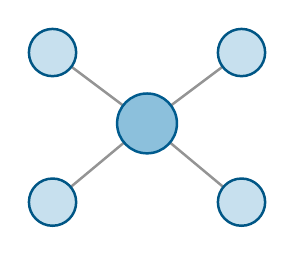
\begin{tikzpicture}[line width=0.9pt]
  % node positions: a central hub with four peers
  \coordinate (c)  at (1.2,1.0);
  \coordinate (n1) at (0,1.9);
  \coordinate (n2) at (2.4,1.9);
  \coordinate (n3) at (0,0);
  \coordinate (n4) at (2.4,0);
  % links
  \foreach \n in {n1,n2,n3,n4}{ \draw[otgray!65] (c) -- (\n); }
  % peer nodes
  \foreach \n in {n1,n2,n3,n4}{
    \filldraw[draw=otblue!75!black, fill=otblue!22] (\n) circle[radius=0.3];
  }
  % hub
  \filldraw[draw=otblue!80!black, fill=otblue!45] (c) circle[radius=0.38];
\end{tikzpicture}
\end{document}
